\begin{Example}[mental2]{Mental impairment and parents' SES}
In \exref{ex:mental1} \CA\ was used to explore the relationship between
ratings of the mental health status of young New Yorkers and
their parents' socioeconomic status (SES).
\figref{fig:correses} showed that most of the association in the
table was accounted for by a single dimension along which both factors
were ordered, consistent with the view that mental health increased
in relation to parents' SES.

For comparison, we first fit the independence model with both
\PROC{CATMOD} and \PROC{GENMOD}.
As we expect, this model fits quite badly,
with $\GSQ\ (15) = 47.418$.
\begin{listing}
%include catdata(mental);
proc catmod data=mental;
   weight count;
   model mental*ses = _response_ / noiter noprofile noresponse;
   loglin mental ses / title='Independence';
   run;
\end{listing}
For illustration, the standardized (adjusted) deviance residuals,
$g_i / \sqrt ( 1 - h_i )$
are obtained in the \PROC{GENMOD}
step (named \pname{stresdev} in the \pname{obstats} \Dset),
and used with the \macro{MOSAIC} to produce the mosaic
display shown in the left panel of \figref{fig:mental2}.%
\footnote{To ensure that the the levels of both factors are ordered
correctly, \pname{MENTAL} and \pname{SES} were entered as numeric
variables in the \Dset\ \pname{MENTAL}, and user-formats were used
to provide the character labels shown in \figref{fig:mental2}.
Because \IML\ does not make use of formatted values, the \macro{TABLE}
was used to convert the numeric variables to character.
}
The parameter \pname{cellfill=dev 0.5}
causes the program to write the value of all residuals greater than 0.5
in absolute value in the corresponding tile.
\begin{listing}
proc genmod data=mental;
   class mental ses;
   model count = mental ses / dist=poisson obstats residuals;
   make 'obstats' out=obstats noprint;
run;

%table(data=mental, var=Mental SES, weight=count, char=Y,
       format=mental mental. ses ses., order=data, out=mental2);
data obstats;
   merge mental2 obstats;
%mosaic(data=obstats, vorder=Mental SES, plots=2, split=H V, resid=stresdev,
   title=Mental Impairment and SES: Independence, cellfill=dev 0.5);
\end{listing}
%% two subfig side-by-side
\begin{figure}[htb]
 \begin{minipage}[t]{.49\linewidth}
  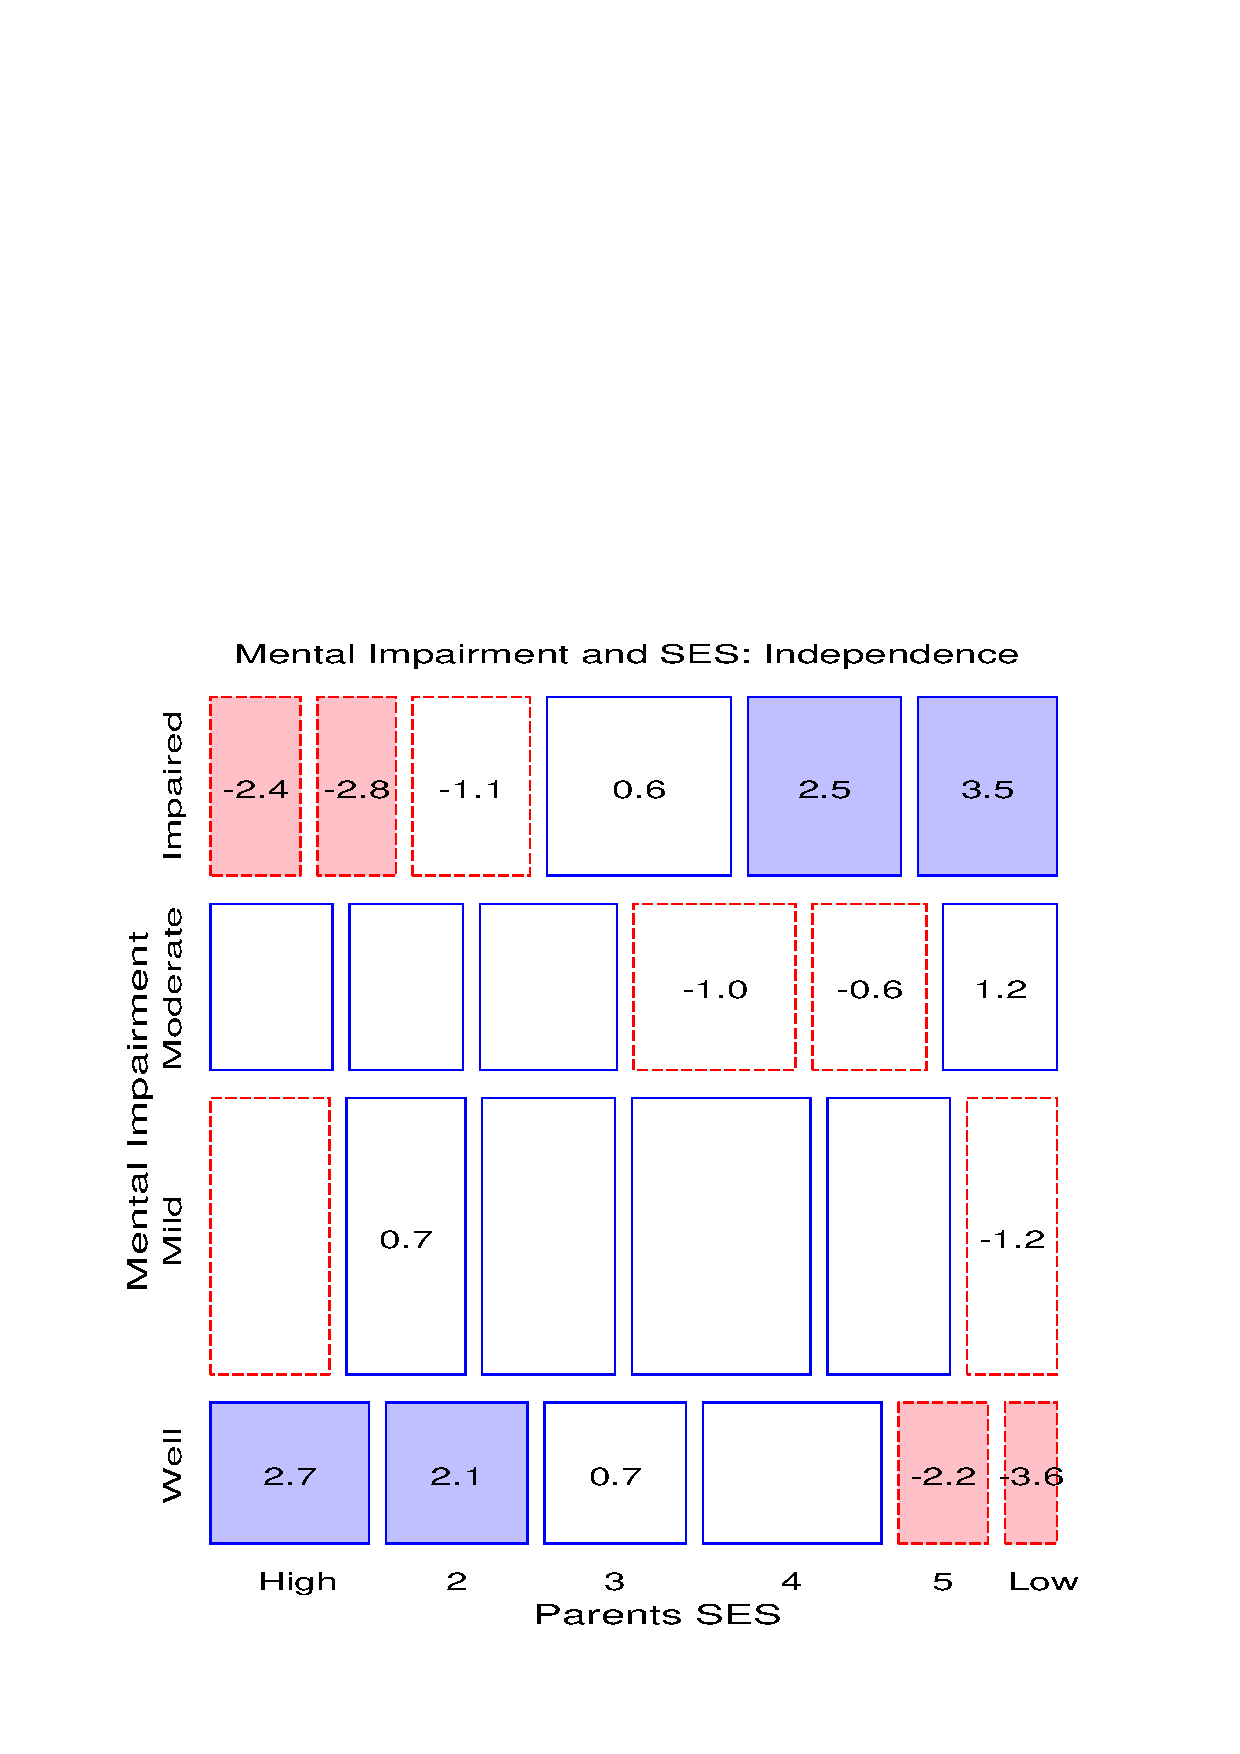
\includegraphics[width=1\linewidth]{mental21}
 \end{minipage}%
 \hfill
 \begin{minipage}[t]{.49\linewidth}
  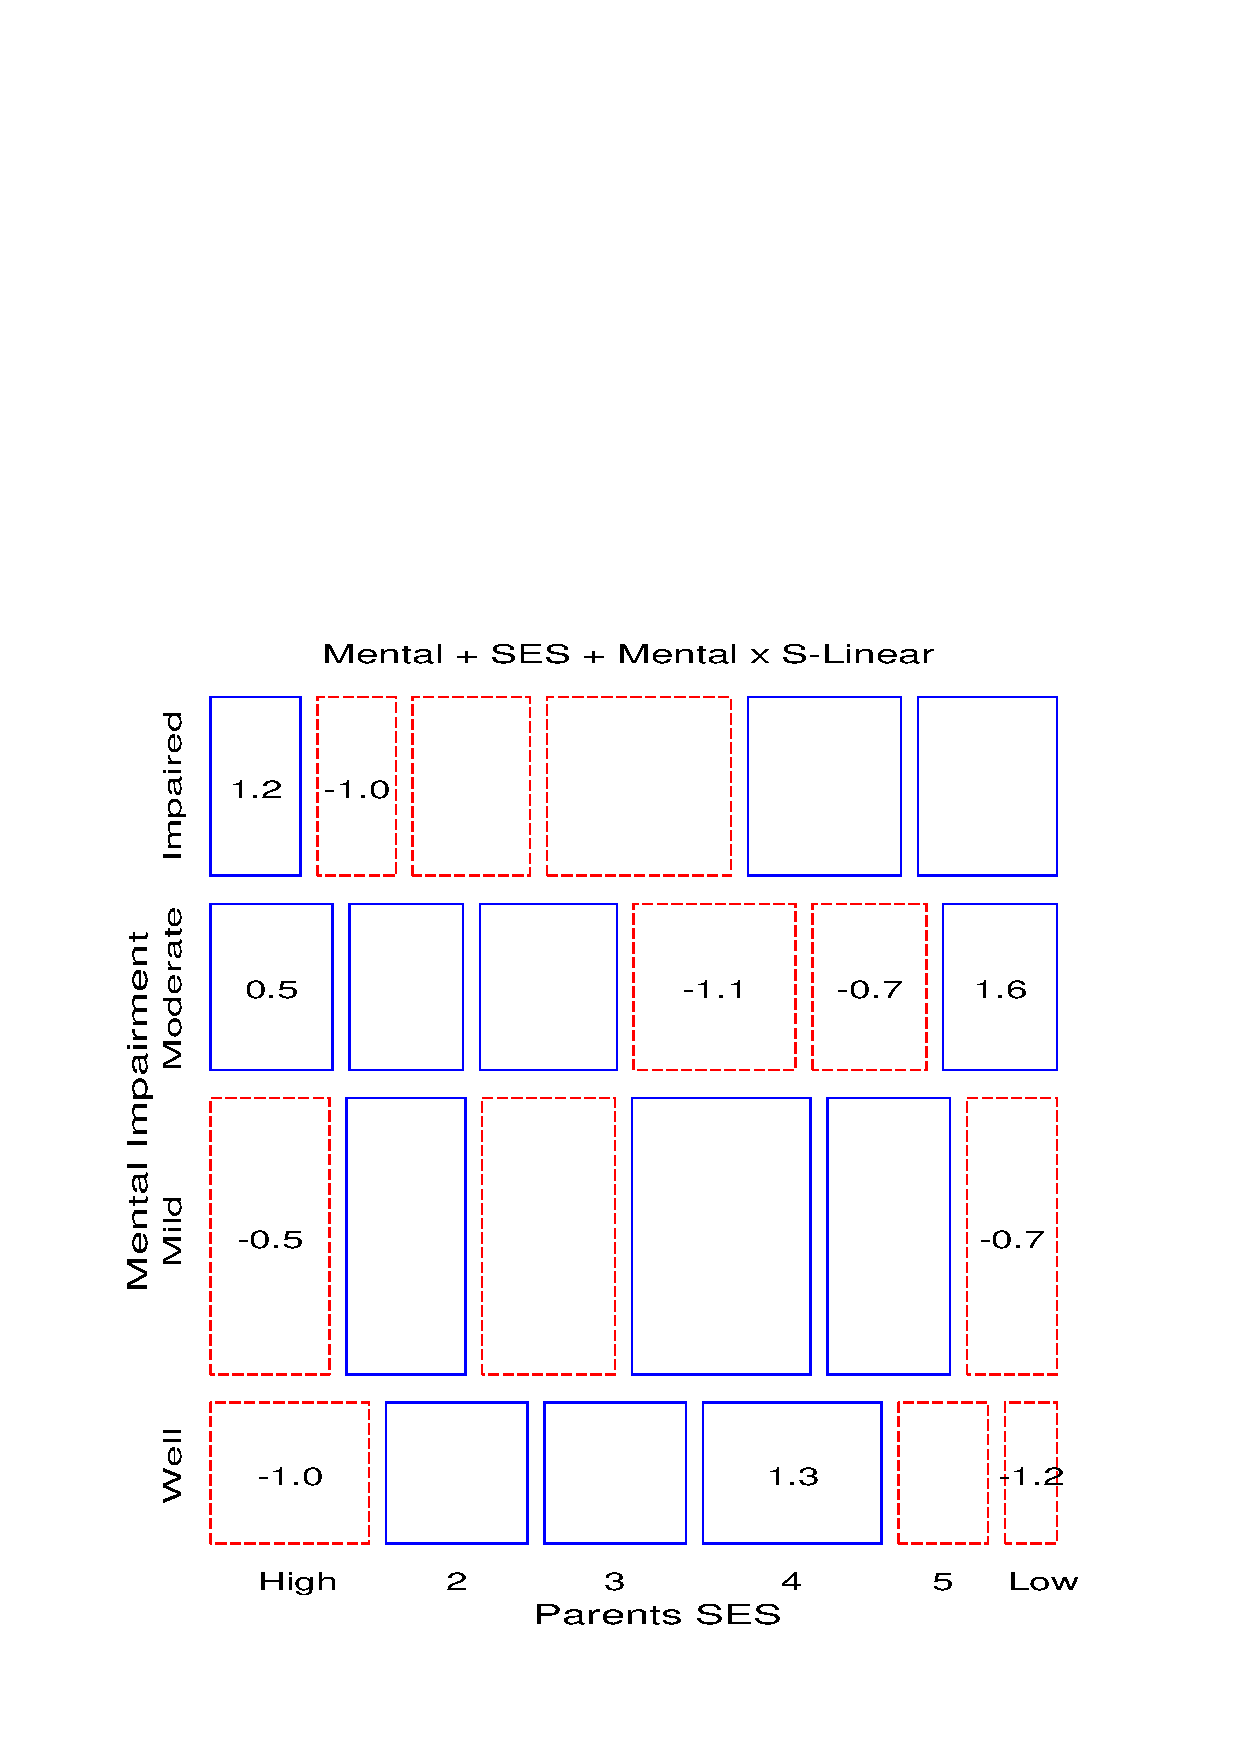
\includegraphics[width=1\linewidth]{mental22}
 \end{minipage}
 \caption[Mental health and SES: Residuals]{Mental health and SES: Residuals from Independence (left) and Row Effects (right) Models}\label{fig:mental2}
\end{figure}
Note that the residuals in \figref{fig:mental2} for the
independence model have the opposite-corner pattern which would
arise if either the row-effects model (with ordered row effects)
or the linear-by-linear
association model described the association between mental health
and SES.
\begin{table}[htb]
 \caption{Mental health data: Goodness-of-fit statistics for ordinal \loglin\ models}\label{tab:mentab2}
 \begin{center}
 \begin{tabular}{l rrrr r}
  \hline
  Model                & df & $\chisq$ & $\GSQ$ & $\Delta \GSQ$  & AIC \\ 
  \hline
  Independence         & 15 & 45.985 & 47.418 & .    &  17.42\\ 
  Linear-by-linear     & 14 & 9.732 & 9.895 & 37.523 & -18.18\\ 
  Row-effects (Mental) & 12 & 6.289 & 6.281 & 41.137 & -17.72\\ 
  \hline
 \end{tabular}
 \end{center}
\end{table}



To fit models in which the association terms for \pname{mental} and/or
\pname{ses} use quantitative scores, create copies, \pname{M} and
\pname{S} of these variables.  They are used as quantitative variables
when they appear in the \stmt{MODEL}{GENMOD}, but are \emph{not} listed
as \pname{CLASS} variables.
The following statements fit the row-effects model, using SES
as a linear effect, and then the linear-by-linear model.
Goodness-of-fit statistics for all three models are shown in
\tabref{tab:mentab2}.

\begin{listing}
data mental;
   set mental;
   m = mental;    *-- copy m and s as quantitative, non-class;
   s = ses;

title 'Linear SES';
proc genmod data=mental;
   class mental ses;
   model count = mental ses mental*s / dist=poisson obstats residuals;
   make 'obstats' out=obstats noprint;
run;
data obstats;
   merge mental obstats;
%mosaic(data=obstats, var=Mental SES, resid=stresdev,  split=H V,
   title=Mental + SES + Mental x S-Linear, cellfill=dev 0.5);

title 'Linear x Linear';
proc genmod data=mental;
   class mental ses;
   model count = mental ses m*s / dist=poisson obstats residuals;
run;
\end{listing}
The $\Delta \GSQ$ values in \tabref{tab:mentab2} each test whether
the corresponding model results in a significant reduction in the
residual $\GSQ$ compared to the independence model.  Both are
highly significant.

Similarly, the difference in $\GSQ$ between the linear-by-linear
and row-effects model, $\Delta \GSQ\ (2) = 9.732-6.289 = 3.443$ suggests that the 
row-effects model
is \emph{not} a significant improvement over the
linear-by-linear model.
The AIC values suggest a slight preference for the linear-by-linear model.
The residuals for the row effects model are shown in the right
panel of \figref{fig:mental2}; residuals for the linear-by-linear
model (not shown) have the same signs, but are slightly smaller
in some cells.

\begin{Output}[htb]
\caption{Parameter estimates for the row-effects \loglin\ model, Mental health data}\label{out:mental2.1}
\small
\verbatiminput{ch7/out/mental2.1}
\end{Output}

Under the linear-by-linear model, the estimate of the coefficient of
\pname{M*S} is $\hat{\gamma} = 0.0907$ (s.e.=0.015) with unit-spaced scores.
This corresponds to a local odds ratio, $\hat{\theta}_{ij} = \exp (0.0907) = 1.095$.
This single number describes the association succinctly:
each step down socioeconomic scale increases the odds of being classified
one step poorer in mental health by 9.5\%.

Parameter estimates for the row-effects model are shown in
\outref{out:mental2.1}.  The row effects are the values of
the \pname{S*MENTAL} terms.  These values are ordered, consistent with
mental health status having ordinal associative effects,
but (with integer scores for both variables) they are not equally
spaced, as the linear-by-linear model would imply.
The spacing of these parameter estimates is similar to what we saw
in the \CA\ plot (\figref{fig:correses}), with the middle categories
Mild Impairment, and Moderate Impairment relatively close together
compared to the extreme categories.

These \loglin\ models and the associated mosaic displays do not
provide a clear preference between the row-effects and linear-by-linear
models here.
We turn now to other models and graphical displays which may distinguish them better.
\end{Example}
